% !TEX root = ./docs.tex

\subsection{Grafische Oberfläche bei den Nutzern}
Wählt der Nutzer nach dem Starten des Clients die Variante mit Grafischer Benutzeroberfläche starten, ruft der Client die Methode startGui() auf. Hierbei wird ein JFrame erzeugt, auf dem im Laufe der Zeit unterschiedliche JPanels hinzugefügt und entfernt werden. Je nachdem an welchem Punkt der Nutzer sich gerade befindet werden die entsprechenden Methoden wie loginPanel() oder displayRecentConversations() für die jeweilige Funktionalität aufgerufen. \\ \\
//TODO: Erkläen: Wie bekommt die GUI neue Chatnachrichten (eigener "Listener" Thread) \\
//TODO (Wenn noch Platz vorhanden): startGui() erklären wie Daten aus Entites gelesen wird
\subsection{Verwendung von Emojis}
Hier haben wir es uns zu nutze gemacht, dass die meisten gängigen Emojis bereits als Unicode Zeichen vorhanden sind. Durch das Verwenden der Unicode Zeichen kann eine zu versenden Nachricht weiterhin als String an eine Message Entität übergeben werden. Java wandelt den Unicode automatisch in das zugehörige Emoji um, sodass keine Icons für die Emojiauswahl oder weitere Anpassungen im Frontend nötig waren. Bei der Auswahl eines Emojis wird ein Objekt der Klasse EmojiMouseListener instanziiert, welches den entsprechenden Unicode Wert an die JTextArea anhängt. So ist es jederzeit möglich die Anzahl der Emojis zu erhöhen oder Emojis zu tauschen, indem das Gridlayout welches die Methode renderEmojiPanel() liefert angepasst wird.

Auf Serverseite mussten hierfür keine Veränderungen vorgenommen werden.

\subsection{Mehrere Chatverläufe pro Nutzer}
//TODO

\subsection{Gruppenchats}
Gruppenchats stellen nur eine Erweiterung der bestehenden Chatimplementierung dar. Statt das ein Chat nur die beiden Teilnehmer besitzt, besitzt es nur beliebig viele Nutzer. Wird eine Nachricht empfangen werden nun alle am Chatbeteiligten Nutzer durchlaufen und die Nachricht wird an alle der Node bekannten Clients weitergeleitet. Außerdem wird wie bereits erwähnt die Nachricht aus Konsistenzgründen weiter gebroadcastet.

\subsection{Persistentes Speichern der Chatverläufe}
Sämtliche der Node bekannten Informationen (Nutzer, Chats, Nachrichten) werden in einem Warehouse verwaltet. Um diese Informationen zwischen Node-Neustarts zu persistieren muss demnach das Warehouse als Datei gespeichert werden und bei Node-Start wieder geladen werden. Existiert noch kein Speicherstand wird die Node mit einem leeren Warehouse initialisiert. Während die Node ausgefallen ist, können andere Nodes gleichzeitig neue Informationen erhalten haben. Sobald die Node wieder verfügbar ist müssen andere Nodes dies bemerken und die ausgefallene Node mit Informationen versorgen. Um den Ausfall festzustellen ist ein Heart-Beat vorgesehen. Dieser pingt jede Sekunde alle benachbarten Nodes an um sicherzustellen, dass die Verbindung noch existiert. Sollte eine Unterbrechung festgestellt, versucht die Node die Verbindung wieder aufzubauen. Gelingt dies, so wird das Warehouse übersendet. Jede Node prüft ob sie alle Informationen des empfangenen Warehouses bereits besitzt und fügt neue Informationen hinzu. Sofern die Node neue Informationen erhalten haben, broadcastet diese ihren neuen Stand an alle benachbarten Nodes um diese auch auf den neuesten Stand zu bringen.

Der Speichervorgang kann je nach System und Warehousegröße längere Zeiten in anspruch nehmen. In dieser Zeit können in der Regel keine weiteren Anfragen verarbeitet werden. Um diese Zeit zu minimieren kümmert sich ein eigener Thread um die Speicherung und speichert das Warehouse in Intervallen.
Zu beachten ist der Fall, dass eine Node zusammenbricht während der Speichervorgang in Arbeit ist. In diesem Fall würde die node sämtliche Informationen verlieren, da die Speicherdatei korrupt ist. Um dies zu verhindern wird der Speicherstand zunächst in eine Tempdatei geschrieben und nach erfolgreicher speicherung an den Zielort verschoben.

\subsection{Verschlüsselte Übertragung der Chat-Nachrichten}
Um einen sicheren Nachrichtenkanal zu gewährleisten wurde eine 
Ende-zu-Ende-Verschlüsselung implementiert. Dabei wird beim
erstellen eines Chats unter allen Teilnehmern ein Diffie-Hellman 
Schlüsselaustausch durchgeführt, sodass jeder Client denselben 
Schlüssel für einen Chat besitzt. Diese generierten Schlüssel 
werden beim Client zur Chat ID lokal gespeichert, sodass der
Server die Schlüssel nie kennen wird. Somit kann der Client,
bevor er Nachrichten zum Server sendet den Inhalt mit dem 
jeweiligen Chat Schlüssel verschlüsseln und ankommenende 
Nachrichten entschlüsseln.

Um auch Gruppenchats ermöglichen zu können musste der 
Diffie-Hellman-Schlüsselaustausch entsprechend erweitert werden.
Dabei gibt es in Gruppen im Gegensatz zu zwei Teilnehmern 
mehrere Runden. Ein Schlüsselaustausch mit drei Teilnehmern kann
aus dem untererem Schaubild entnommen werden:

\begin{figure}[h]
  \centering
  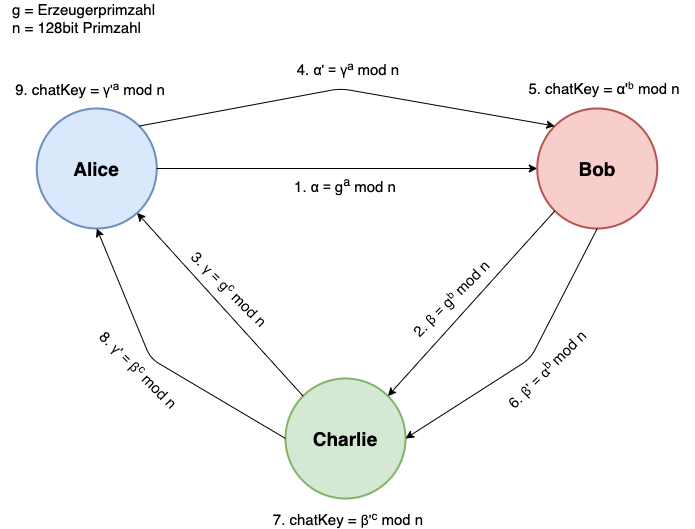
\includegraphics[width=\textwidth]{dh.png}
  
  \caption{Erweiterter Diffie-Hellman}
  \label{}
\end{figure}

Wie man erkennen kann werden in der ersten Runde (Schritte 1-3)
die ersten Teilschlüssel wie im klassischen Diffie-Hellman generiert
und weitergeschickt. In der zweiten Runde wird mithilfe der Ergebnisse
der ersten Runde die fertigen Chat Schlüssel berechnet (Schritte 4-9).
Dieses Verfahren kann mit beliebig vielen Teilnehmern durchgeführt
werden, jedoch steigt die Anzahl der Runden linear und die Anzahl der 
Requests quadratisch.

$$ rounds = n - 1 $$
$$ requests = n \cdot (n - 1) $$

Wobei hier n die Anzahl der Teilnehmer ist.

Da nun alle Chatteilnehmer den gleichen Schlüssel besitzen und dieser 
lokal gesichert ist können Nachrichten mit einem symetrischen Verfahren
sicher versendet werden.

\subsection{Verschlüsselte serverseitige Speicherung der Chats}
//TODO

%\subsection{3 replizierte Server mit Majority Consensus Strategie}
% Gibt in unserem Ansatz keinen Sinn
